\documentclass{article}

\usepackage{tikz}

\begin{document}

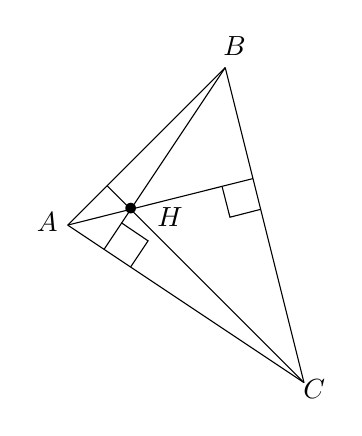
\begin{tikzpicture}
  % Triangle
  \draw (0,0)-- (2,2); % [AB]
  \draw (2,2)-- (3,-2); % [BC]
  \draw (0,0)-- (3,-2); % [AC]
  % Hauteurs
  \draw (2,2)-- (0.46,-0.31); % hauteur B
  \draw (0,0)-- (2.35,0.59); % hauteur A
  \draw (3,-2)-- (0.5,0.5); % hauteur C
  % Etiquettes des sommets
  \draw (-0.26,0.04) node {$A$};
  \draw(2.12,2.27) node {$B$};
  \draw (3.13,-2.08) node {$C$};
  % angles droits
  \draw (1.96,0.49) -- (2.06,0.1) -- (2.45,0.2) ; % sur [BC]
  \draw (0.8,-0.53) -- (1.02,-0.2) -- (0.68,0.03); % sur [AC];
  % Orthocentre
  \draw (0.8,0.2) node{$\bullet$} +(0.5,-0.1) node{$H$};
\end{tikzpicture}

\end{document}
